\section{提案} \label{sec:proposal}

\subsection{概要}

本論文では,Unikernel の \rr を効率的に行う \emph{\sysname}を紹介する.
\sysname の設計目標は以下のとおりである.

\begin{itemize}
    \item \textbf{Unikernel レイヤのみの Reboot-based Recovery.}{\sysname は,従来の Unikernel の再起動とは異なり,アプリケーションのメモリの内容を保持したまま Unikernel のメモリを若返らせる.アプリケーションは,私たちの Unikernel の再起動に渡って,継続して動作することができる.}
    \item \textbf{特定の Unikernel の構成に依存しない.}{特定の Unikernel のコンポーネントに依存する \rr のメカニズムは,Unikernel の構成がアプリケーションごとに異なるためアプリケーションごとの再設計が必要となり,合理的ではない.提案手法は,どのような Unikernel のコンポーネントにも適用できる.}
    \item \textbf{ダウンタイムをできるだけ短くする.}{\sysname は Unikernel の再起動によるアプリケーションのダウンタイムをできる限り短縮する.}
\end{itemize}

\begin{figure}[t]
    \begin{center}
      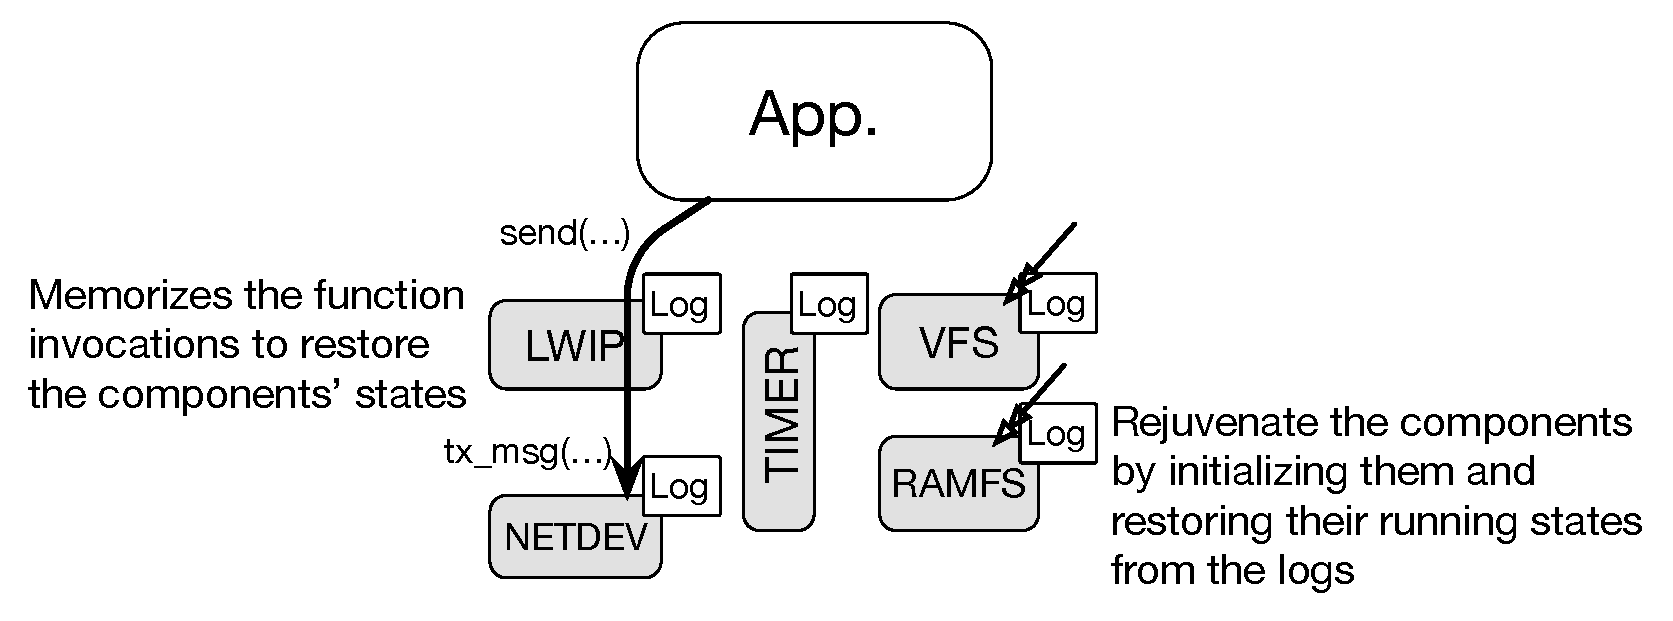
\includegraphics[scale=0.3]{./img/vampos.eps}
      \caption{{\sysname} の概要} 
      \label{fig:overview}
    \end{center}
\end{figure}

これらの目標を達成するために,\sysname は Unikernel のカスタマイズ性を利用している.
Unikernel は多数のコンポーネントを提供し,
コンポーネント間のインタフェースが明確に定義されているため,
アプリケーションの動作に必要なコンポーネントのみを選択することができる.
\sysname の概要を図\ref{fig:overview}に示す.
\sysname はコンポーネント単位での Unikernel の再起動を可能にし,
リンクしたアプリケーションを継続して実行できるように,
再起動したコンポーネントの動作状態を復元する.
具体的には,\sysname は,公開されているコンポーネントインタフェースをフックすることにより,コンポーネント間のインタラクションを記録し,
ログを再生することで,状態を持つコンポーネントの動作状態を復元する.
たとえば,ファイルシステムの再起動においては,\sysname は,
他のコンポーネントの動作状態の変更しないように,
そのコンポーネントのみを再起動し,再起動したコンポーネント内部でログを再生する.

また,\sysname では,\rr による Unikernel の再起動の効果を最大化するために,
コンポーネント間のエラー伝搬を防止する.
コンポーネントのフォルトが別のコンポーネントへと伝搬することで,
複数のコンポーネントで連鎖的にフォルトが発生してしまうが,
コンポーネント単位での再起動では,
一度に一つのコンポーネントのエラー状態しか解消することができない.
そのような場合,
Unikernel 全体を安定化させるためには,
フォルト状態にあるコンポーネントすべての再起動の完了を待つ必要があり,
不安定な状態が慢性化する可能性がある.

\sysname の目標は,\rr の効果を得ることであり,通常の再起動との完全な互換を目指しているわけではない.
Unikernel がリンクしたアプリケーションの再起動して Unikernel を若返らせるのではなく,
代わりに \sysname の再起動を実行すればよい.
\sysname のメカニズムは,
通常の再起動によるソフトウェアアップデートや再構成のような他の目的に適用するものではなく,
そのような目的のためには通常の再起動が使われる.

\sysname の設計は以下の技術的な課題を提示する.
(1)どのように,Unikernel をコンポーネント単位で若返らせるのか?
(2)どのように,対象のコンポーネントのみを復元するのか?
(3)どのように,再起動したコンポーネントの状態を効率良く復元するのか?
(4)どのように,コンポーネント間を分離するのか?
次の章では,これらの課題に対する解決策を述べる.
以下の議論は Unikraft~\cite{KuenzerEtAl-Unikraft} 上のプロトタイプの開発に基づくものであるが,
IncludeOS~\cite{BratterudEtAl-IncludeOS} のような他の Unikernel にも十分に適用できる一般性を持つであろう.
